\documentclass{exam}
\usepackage[utf8]{inputenc}
\usepackage{lmodern}
\usepackage{microtype}

% \usepackage[parfill]{parskip}
\usepackage[dvipsnames]{xcolor}
\usepackage{amsmath}
\usepackage{amsfonts}
\usepackage{amsthm}
\usepackage{siunitx}
\DeclareSIUnit\year{yr}
\DeclareSIUnit\foot{ft}
\DeclareSIUnit\litre{\liter}

\usepackage{skull}

\usepackage{pgfplots}
\usepgfplotslibrary{polar}
\pgfplotsset{compat=1.11}
\usepgfplotslibrary{statistics}
\usepackage{graphicx}
\usepackage{sidecap}
\sidecaptionvpos{figure}{c}
\usepackage{float}
\usepackage{gensymb}
\usepackage{tkz-euclide}
\usetkzobj{all}
\usepackage{commath}
\usepackage{hyperref}
\usepackage{enumitem}
\usepackage{wasysym}
\usepackage{multicol}
\usepackage{mathtools}
\usepackage{tcolorbox}
\usepackage{tabularx}
\usepackage[version=4]{mhchem}
\usepackage{changepage}
\usepackage{listings}
\lstset{basicstyle=\ttfamily\linespread{0.8}\small}

\renewcommand*{\thefootnote}{\fnsymbol{footnote}}

\newtheorem*{thm}{Theorem}
\newtheorem*{iden}{Identity}
\newtheorem*{lemma}{Lemma}
\newtheorem{obs}{Observation}
\theoremstyle{definition}
\newtheorem*{defn}{Definition}
\newtheorem*{ex}{Example}
\newtheorem{con}{Construction}
\newtheorem*{alg}{Algorithm}

\newtheoremstyle{break}
  {\topsep}{\topsep}%
  {\itshape}{}%
  {\bfseries}{}%
  {\newline}{}%
\theoremstyle{break}
\newtheorem*{bthm}{Theorem}

% russian integral
\usepackage{scalerel}
\DeclareMathOperator*{\rint}{\scalerel*{\rotatebox{17}{$\!\int\!$}}{\int}}

% \DeclareMathOperator*{\rint}{\int}

\pgfplotsset{vasymptote/.style={
    before end axis/.append code={
        \draw[densely dashed] ({rel axis cs:0,0} -| {axis cs:#1,0})
        -- ({rel axis cs:0,1} -| {axis cs:#1,0});
    }
}}

% \pointsinrightmargin
\boxedpoints
\pointname{}

\newcommand{\questioA}{\question[\texttt{\textbf{\color{Cerulean} A}}]}
\newcommand{\questioM}{\question[\texttt{\textbf{\color{PineGreen} M}}]}
\newcommand{\questioE}{\question[\texttt{\textbf{\color{WildStrawberry} E}}]}
\newcommand{\questioS}{\question[\texttt{\textbf{\color{Goldenrod} S}}]}
\newcommand{\questioO}{\question[\texttt{\textbf{\color{BurntOrange} O}}]}

\newcommand{\parA}{\part[\texttt{\textbf{\color{Cerulean} A}}]}
\newcommand{\parM}{\part[\texttt{\textbf{\color{PineGreen} M}}]}
\newcommand{\parE}{\part[\texttt{\textbf{\color{WildStrawberry} E}}]}
\newcommand{\parS}{\part[\texttt{\textbf{\color{Goldenrod} S}}]}
\newcommand{\parO}{\part[\texttt{\textbf{\color{BurntOrange} O}}]}

\newcommand{\subparA}{\subpart[\texttt{\textbf{\color{Cerulean} A}}]}
\newcommand{\subparM}{\subpart[\texttt{\textbf{\color{PineGreen} M}}]}
\newcommand{\subparE}{\subpart[\texttt{\textbf{\color{WildStrawberry} E}}]}
\newcommand{\subparS}{\subpart[\texttt{\textbf{\color{Goldenrod} S}}]}
\newcommand{\subparO}{\subpart[\texttt{\textbf{\color{BurntOrange} O}}]}

\newcommand{\mainHeader}[2]{\section*{NCEA Level 2 Mathematics\\#1. #2}}
\newcommand{\mainHeaderHw}[2]{\section*{NCEA Level 2 Mathematics (Homework)\\#1. #2}}
\newcommand{\seealso}[1]{\begin{center}\emph{See also #1.}\end{center}}
\newcommand{\drills}[1]{\begin{center}\emph{Drill problems: #1.}\end{center}}
\newcommand{\basedon}[1]{\begin{center}\emph{Notes largely based on #1.}\end{center}}

\begin{document}

\mainHeaderDiff{13}{Sequences and Series}
\goals{To revise last year's material on sequences, especially how they behave `at infinity'.}
\subsection*{Sequences}
So far, we have looked at functions that are continuous. This week, we take a short break from this and look at sequences and series. A sequence
is, intuitively, a list of numbers written in a definite order:
\begin{displaymath}
  (a_n) = (a_1, a_2, \dots, a_i, \dots).
\end{displaymath}
Note that we index sequences starting at 1, unless stated otherwise. Theoretical computer scientists will often start at 0 instead.

Some examples of sequences include
\begin{gather}
  \left(n\right) = (1,2,3,\dots) \text{}\\
  \left(\frac{n-1}{n}\right) = \left(0,\frac{1}{2},\frac{2}{3},\frac{3}{4},\dots\right)\\
  \left(\cos \frac{n\pi}{6} \right) = \left(1, \frac{\sqrt{3}}{2}, \frac{1}{2}, 0, \dots\right)\\
  \left(1 - 0.2^n \right) = \left(0.8, 0.96,0.992,0.9984,\dots \right)\\
  \left(\frac{n^5}{n!}\right) = \left(0, 1, 16,40.5,42.6,26.04,10.8,\dots\right)\\
  \left( a_n \right) = \left(1,0,1,0,0,1,0,0,0,1,\dots\right)
\end{gather}
Clearly some of these sequences grow forever, while others settle down and become closer and closer to a particular value.
\begin{defn}
  A sequence $ (a_n) $ has a limit $ L $, written $ \lim_{n\to\infty} a_n = L $, if we can make the terms $ a_i $ stay as close as we like
  to $ L $ by taking $ i $ sufficiently large. If $ (a_n) $ has a limit, then it is called \textbf{convergent}; otherwise, it is
  called \textbf{divergent}.
\end{defn}

Examples (2) and (4) above are clearly convergent (they both converge to 1); example (5) is convergent to 0, even though it is initially
increasing (because factorials grow faster than powers eventually). The others are all divergent:
\begin{enumerate}
  \item[(1)] is clearly divergent because as $ n \to \infty $, $ a_n \to \infty $.
  \item[(3)] is divergent because there is no number $ L $ such that $ a_i $ stays close to $ L $ as we increase $ i $ (it always jumps around).
  \item[(6)] is divergent for the same reason as (3).
\end{enumerate}

Some sequences can be written recursively.
\begin{gather*}
  a_1 = 1, a_{n + 1} = 5a_n - 3 \quad (1, 2, 7, \dots)\\
  a_1 = 2, a_{n + 1} = \frac{a_n}{1 + a_n} \quad \left(2, \frac{2}{3}, \frac{2}{5}, \frac{2}{7}, \dots\right)
\end{gather*}

\begin{ex}
  The \textbf{Fibonacci} sequence is defined by
  \begin{displaymath}
    (F_i) = \begin{cases}
      1 & \text{if $ i = 1 $ or $ i = 2 $,}\\
      F_{i - 1} + F_{i - 2} & \text{otherwise.}
    \end{cases}
  \end{displaymath}
  The first few elements of the Fibonacci sequence are 1, 1, 2, 3, 5, 8, 13, 21.

  There is actually a closed-form formula for the Fibonacci sequence:
  \begin{displaymath}
    F_i = \frac{\left(1 + \sqrt{5}\right)^n - \left(1 - \sqrt{5}\right)^n}{2^n \sqrt{5}}.
  \end{displaymath}
  More information about this sequence is given in the reading for the homework.
\end{ex}

\subsection*{Series}
From sequences, we move on to infinite sums (also known as series). Given some sequence $ (a_n) $, we have a series
\begin{displaymath}
  \sum_{n = 1}^\infty a_n = a_1 + a_2 + a_3 + \cdots.
\end{displaymath}

Often it does not make sense to talk about the sum of infinitely many terms; obviously $ 1 + 2 + 3 + \cdots $ will increase
forever. On the other hand, if we add the first $ n $ terms of
\begin{displaymath}
  \left(\frac{1}{2}, \frac{1}{4}, \dots, \frac{1}{2^n}, \dots\right)
\end{displaymath}
we obtain $ 1 - 1/2^n $, which converges to 1.

This suggests that we can consider the partial sums of a sequence $ (a_n) $
\begin{align*}
  s_1 &= a_1\\
  s_2 &= a_1 + a_2\\
  s_3 &= a_1 + a_2 + a_3\\
      &\vdotswithin{=}\\
  s_n &= a_1 + \cdots + a_n = \sum_{i = 1}^n a_n
\end{align*}
and then say that the sum $ \sum a_n $ exists if the sequence $ (s_n) $ converges.

An important class of series is the geometric series
\begin{displaymath}
  \sum_{n = 1}^\infty ar^{n - 1} = a + ar + ar^2 + \cdots
\end{displaymath}
where $ a \neq 0 $ and $ r $ are constants. Clearly if $ \abs{r} \geq 1 $ then the sum becomes $ a + a + \cdots $ which converges;
if $ \abs{r} < 1 $, then we have
\begin{align*}
  s_n  &= a + ar + ar^2 + \cdots + ar^{n - 1}\\
  rs_n &= \phantom{a + {}} ar + ar^2 + ar^3 + \cdots + ar^n\\
  s_n - rs_n &= a - ar^n\\
  s_n = \frac{a - ar^n}{1 - r}.
\end{align*}
which converges to $ a/(1-r) $ as $ n \to \infty $; so the sum exists.

\subsection*{Questions}
\begin{questions}
  \questioM Which of the following sequences are convergent (write the limit), and which are divergent (give a reason)?
    \begin{parts}
      \part $ ((-1)^n) $
      \part $ (e^{1/n}) $
      \part $ (n^2 e^{-n}) $
      \part $ (3^n/(1+2^n)) $
      \part $ a_1 = 6 $, $ a_{n + 1} = a_n/n $
      \part $ (\cos 2\pi/n) $
      \part $ (\sin n!/n^n) $
      \part $ (\sin n^n/n!) $
    \end{parts}
  \questioE Find the limit of the sequence $ (\sqrt{2}, \sqrt{2\sqrt{2}}, \sqrt{2\sqrt{2\sqrt{2}}}, \dots) $.
  \questioA Find the sum of the geometric series $ 1 + 1/2 + 1/4 + \cdots $.
  \questioM Find the sum of the geometric series $ 5 - \frac{10}{3} + \frac{20}{9} - \frac{40}{27} + \cdots $.
  \questioE Show that the series $ \sum_{n = 1}^{\infty} \frac{1}{n(n + 1)} $ is convergent, and find its sum. [Hint: calculate $ \frac{1}{i} - \frac{1}{1 + i} $.]
  \questioE Determine whether $ \sum_{n =1}^\infty \ln \frac{n}{n + 1} $ is convergent or divergent. If it is convergent, find its sum.
  \questioE Consider the harmonic series
            \begin{displaymath}
              \sum_{n = 1}^\infty \frac{1}{n} = 1 + \frac{1}{2} + \frac{1}{3} + \cdots.
            \end{displaymath}
    \begin{parts}
      \part Let $ s_n $ be the sequence of partial sums. Show that $ s_4 = 1 + \frac{1}{2} + \frac{1}{3} + \frac{1}{4} > 1 + \frac{2}{2} $ [Hint: $1/3 > 1/4$.]
      \part Show that $ s_8 > 1 + \frac{3}{2} $.
      \part Prove that $ s_{2^n} \geq 1 + \frac{n}{2} $ in general. Conclude that the harmonic series diverges.
    \end{parts}
  \questioE Find $ c $ if $ \sum_{n = 1}^\infty (1 + c)^{-n} = 2 $.
  \questioS A power series is a series of the form
            \begin{displaymath}
              \sum_{n = 0}^{\infty} c_n x^n = c_0 + c_1 x + c_2 x^2 + \cdots.
            \end{displaymath}
            You can think of a power series as a polynomial with infinitely many terms. It can be shown that the normal sum rule for differentiation holds,
            so that $ \od{}{x} \sum_{n = 0}^{\infty} c_n x^n = \sum_{n = 0}^{\infty} \od{}{x} c_n x^n $.
    \begin{parts}
      \item Find the derivative of the Bessel function, $ J_0(x) = \sum^{\infty}_{n = 0} \dfrac{(-1)^n x^{2n}}{2^{2n} (n!)^2} $.
      \item If $ \abs{x} < 1 $, show that $ \sum_{n = 0}^\infty x^n = \frac{1}{1 - x} $.
      \item Find a power series representation for $ f(x) = 1/(1-x)^2 $. [Hint: differentiate the equation in (b).]
      \item Find a power series representation for $ g(x) = \ln(1 + x) $. [Hint: differentiate $ g $, use (c), and antidifferentiate.]
      \item When is the power series representation of $ g $ valid?
    \end{parts}
  \questioS The Cantor set is constructed as follows. Start with the closed interval $ [0,1] $ and remove the open interval $ (\frac{1}{3}, \frac{2}{3}) $. This leaves
            the two closed intervals $ [0, \frac{1}{3}] $ and $ [\frac{2}{3},1] $; remove the open middle third of each of these. Four intervals remain; remove the
            open middle third of each. Continue this process indefinitely, at each step removing the open middle third of each interval remaining from the previous
            step. The Cantor set is the set of numbers remaining from the interval $ [0,1] $ after this process has been carried out.
            \begin{center}
              
\includegraphics[width=0.6\textwidth]{cantor}
            \end{center}
    \begin{parts}
      \part Show that the total length of all the removed intervals is 1.
      \part Despite this, there are still infinitely many numbers remaining. Exhibit some members of the Cantor set.
      \part The Sierpinski carpet is a two-dimensional version of the Cantor set; remove the centre one-ninth of a square of side 1, then the centres
            of the eight remaining squares, and so on. Show that the sum of the areas of the removed squares approaches 1. Hence the Sierpinski carpet
            has area zero.
            \begin{center}
              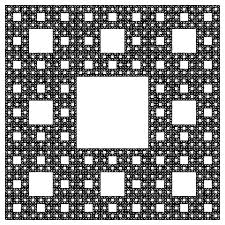
\includegraphics[width=0.3\textwidth]{sierpinski}
            \end{center}
    \end{parts}
  \questioS Scholarship 2017: The sequence $ (a_n) $ is defined as follows:-
            \begin{displaymath}
            \begin{cases}
              (a_1) = 2,\\
              (a_2) = 7,\\
              (a_{n + 1}) = \frac{1}{2}(a_n + a_{n + 1}) & \text{ for $ n \geq 2 $.}
            \end{cases}
            \end{displaymath}
    \begin{parts}
      \part Find an exact formula for the $ n$th term of the sequence.
      \part What is the limit of $ a_n $ as $ n \to +\infty $?
    \end{parts}
  \clearpage
  \questioS Consider the following limit (you may assume that it exists):
            \begin{displaymath}
              L = 0.999... = \lim_{n \to \infty} \sum^n_{i = 0} \frac{9}{10^i}
            \end{displaymath}
    \begin{parts}
      \part Write $ L = 0.9 + 0.09 + \cdots $, and make a conjecture about the value of $ L $.
      \part Prove or disprove your conjecture from (a).
    \end{parts}
  \questioS Zeno was a Greek philosopher active in the 5th century BCE. He presented a list of `paradoxes', or apparent contradictions,
            including the following (adapted from Wikipedia):
            \begin{itemize}
              \item Suppose Achilles is in a foot race with a tortoise. Achilles runs much faster than the tortoise, but the latter
                    has a head start. By the time Achilles reaches the location that the tortoise started, the tortoise will have moved
                    a small amount further on; similarly, by the time Achilles reaches the new location of the tortoise, it will have moved
                    an even smaller distance further on; and by this reasoning it follows that Achilles can never overtake the tortoise.
                    \begin{center}
                      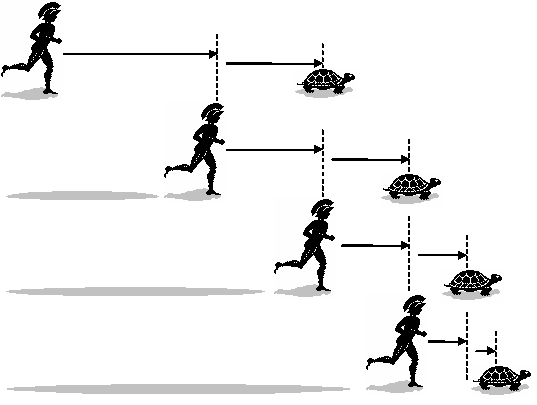
\includegraphics[width=0.4\textwidth]{achilles}
                    \end{center}
              \item Suppose Homer wishes to walk to the end of a path. Before he can get there, he must get halfway there. Before he can
                    get halfway there, he must get a quarter of the way there. Before traveling a quarter, he must travel one-eighth; before
                    an eighth, one-sixteenth; and so on. So Homer cannot walk to the end of the path.
              \item For motion to occur, an object must change the position which it occupies. Consider an example of an arrow in flight. In any
                    one (duration-less) instant of time, the arrow is neither moving to where it is, nor to where it is not. It cannot move to
                    where it is not, because no time elapses for it to move there; it cannot move to where it is, because it is already there.
                    In other words, at every instant of time there is no motion occurring. If everything is motionless at every instant, and
                    time is entirely composed of instants, then motion is impossible.
            \end{itemize}
            Use your knowledge of limits to explain these apparent contradictions.
\end{questions}
\end{document}
